% !TeX encoding = UTF-8
% !TeX program = xelatex
% !TeX spellcheck = en_US

\documentclass[degree=project, degree-type=project]{thuthesis}
  % (DCMMC): add `project` to degree.
  % 学位 degree:
  %   doctor | master | bachelor | postdoc
  % 学位类型 degree-type:
  %   academic(默认)| professional
\usepackage{mathtools}


% 论文基本配置,加载宏包等全局配置
\thusetup{
  output = electronic,
  title = {作业1:方差分析},
  author  = {肖文韬},
  studentid = {2020214245},
  course = {大数据分析},
  include-spine = false,
}

\usepackage{float}
\usepackage{amsthm}
\usepackage[sort]{natbib}
\bibliographystyle{thuthesis-numeric}
\graphicspath{{figures/}}
% hyperref 宏包在最后调用
\usepackage{hyperref}

\begin{document}

% 封面
\maketitle
\frontmatter
% % !TeX root = ../thuthesis-example.tex

% 中英文摘要和关键字

\begin{abstract}
  论文的摘要是对论文研究内容和成果的高度概括。摘要应对论文所研究的问题及其研究目
  的进行描述,对研究方法和过程进行简单介绍,对研究成果和所得结论进行概括。摘要应
  具有独立性和自明性,其内容应包含与论文全文同等量的主要信息。使读者即使不阅读全
  文,通过摘要就能了解论文的总体内容和主要成果。

  论文摘要的书写应力求精确、简明。切忌写成对论文书写内容进行提要的形式,尤其要避
  免“第 1 章……;第 2 章……;……”这种或类似的陈述方式。

  本文介绍清华大学论文模板 \thuthesis{} 的使用方法。本模板符合学校的本科、硕士、
  博士论文格式要求。

  本文的创新点主要有:
  \begin{itemize}
    \item 用例子来解释模板的使用方法;
    \item 用废话来填充无关紧要的部分;
    \item 一边学习摸索一边编写新代码。
  \end{itemize}

  关键词是为了文献标引工作、用以表示全文主要内容信息的单词或术语。关键词不超过 5
  个,每个关键词中间用分号分隔。(模板作者注:关键词分隔符不用考虑,模板会自动处
  理。英文关键词同理。)

  % 关键词用“英文逗号”分隔
  \thusetup{
    keywords = {TeX, LaTeX, CJK, 模板, 论文},
  }
\end{abstract}

\begin{abstract*}
  An abstract of a dissertation is a summary and extraction of research work
  and contributions. Included in an abstract should be description of research
  topic and research objective, brief introduction to methodology and research
  process, and summarization of conclusion and contributions of the
  research. An abstract should be characterized by independence and clarity and
  carry identical information with the dissertation. It should be such that the
  general idea and major contributions of the dissertation are conveyed without
  reading the dissertation.

  An abstract should be concise and to the point. It is a misunderstanding to
  make an abstract an outline of the dissertation and words ``the first
  chapter'', ``the second chapter'' and the like should be avoided in the
  abstract.

  Key words are terms used in a dissertation for indexing, reflecting core
  information of the dissertation. An abstract may contain a maximum of 5 key
  words, with semi-colons used in between to separate one another.

  \thusetup{
    keywords* = {TeX, LaTeX, CJK, template, thesis},
  }
\end{abstract*}


% 目录
% \tableofcontents

% 插图和附表清单
% \listoffigures           % 插图清单
% \listoftables            % 附表清单
% \listoffiguresandtables  % 插图和附表清单

% 正文部分
\mainmatter

\chapter{HW1 ANOVA}

\begin{enumerate}
  \item (\textbf{5 points}) Recall and write down the assumptions which one-way ANOVA are based on.

    ANOVA 是\textbf{方差分析(ANalysis Of VAriance)}的缩写,又称F检验, 用于三个及以上样本均值差别的显著性检验。它基于以下假设:
    \begin{itemize}
      \item 所有的数据都是随机采样的。
      \item 每个组的方差是一样的(同调性),各组的标准差中最大和最小的比例不超过 $2:1$。
      \item 残差是正态分布。
    \end{itemize}
    \vskip 4em

  \item (\textbf{5 points}) Focus on two columns columns: Category (Col[2]) and Average Age (Col[7]). Taking feature Average Age as an example, we want to measure whether the average age varied significantly across the categories. Clearly state the null (H0) and the alternative (H1) hypotheses for this task.

    相同 category 的样本属于同一个组。
    \begin{itemize}
      \item H0: 不是所有组的均值都相等。
      \item H1: 所有组的均值都相等($\mu_1 = \mu_2 = \cdots$)。
     \end{itemize}
    \vskip 4em

\begin{figure}[H]
  \centering
  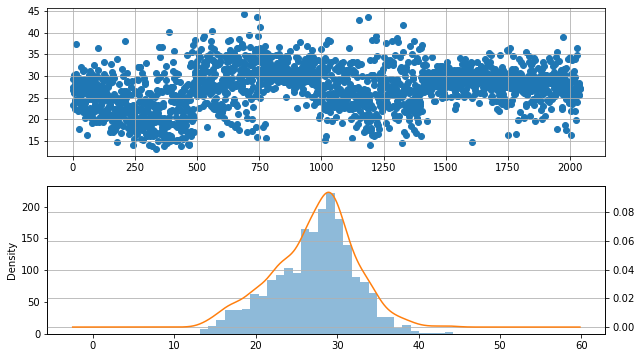
\includegraphics[width=15cm]{col7.png}
  \caption{Col[7]散点图及经验概率密度函数}
  \label{fig:col7}
\end{figure}


   \item Use your favorite statistics analysis software, like Matlab , R, Excel Excel, SPSS or …
     \begin{enumerate}
       \item (\textbf{10 points}) Draw the empirical probability density funfction of Col[7], i.e. the empirical pdf of average age. Does the data in this dimension follow Gaussian distribution? Test normality of Col[7].

         Col[7] 的散点图和经验概率密度函数如图~\ref{fig:col7}所示。
         原假设(H0)假设数据符合正态分布。设置显著性水平 $\alpha = 0.01$,通过计算 p-value $= 4.8348\times 10^{-6} < 0.01$,所以拒绝假设 $H_0$, col[7] 不符合高斯分布.
        \vskip 4em

       \item (\textbf{10 points}) In Col[7], there are 5 components divided by category labels labels. We denote the data in Col[7] with category $i$ (where $i = 1,\cdots,5$) as Col[7|categoty=i]. Test the normality of each components and test the homogeneity of variances.

         设置显著性水平 $\alpha = 0.01$,计算得,组 1,2和3符合正态性,组 4 和 5 不符合正态性。
         同时,计算各组的标准差,最大的与最小的之比为 $2.0437$ 略大于 $2:1$,所以不符合同调性。
         具体计算过程见附件代码。
        \vskip 4em

\begin{figure}[H]
  \centering
  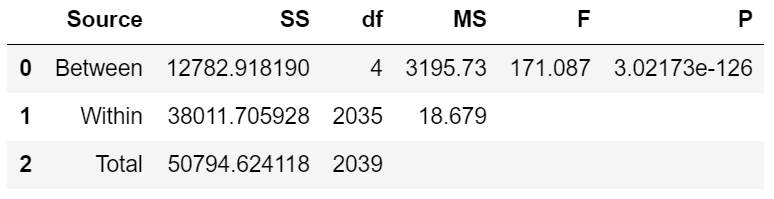
\includegraphics[width=9cm]{col7_ANOVA.png}
  \caption{Col[7]方差分析(ANOVA)}
  \label{fig:col7_anova}
\end{figure}

       \item (\textbf{20 points}) Do the one one-way ANOVA test for Col[7] with categories in Col[2]. Write down your conclusion, supporting statistics, and visualize your data which inspire the process.

         \textbf{结论}:在显著性水平 $\alpha = 0.01$ 下,因为计算得到 p-value $\approx 10^{-126} \ll 0.01$,所以拒绝原假设 $H_0$: 各组的方差相同。
         其计算过程和具体统计量在图~\ref{fig:col7_anova}中展示,具体计算过程见附件代码。
        \vskip 4em
     \end{enumerate}

   \item (\textbf{15 points}) Choose another 3 columns, draw the empirical pdf of each feature columns and test which column follows these assumptions in question 1? How about their corresponding log transformation?
     消息数在取 $\log$ 之后从原来不符合同掉性变为符合同调性,并且原来五个组均不符合高斯分布,变换之后有两个符合高斯分布了。
    \vskip 4em

   \item How to do one one-way ANOVA with the non-normal data data?
     \begin{enumerate}
       \item (\textbf{10 points}) Find and list the possible solutions set.
        \vskip 4em

       \item (\textbf{25 points}) Do the one one-way ANOVA on the 3 columns you choose choose. Do these feature columns vary significantly? Visualize the results.
        \vskip 4em
     \end{enumerate}
\end{enumerate}

% 其他部分
\backmatter

% 参考文献
\bibliography{ref/refs}  % 参考文献使用 BibTeX 编译

% 附录
\appendix
\end{document}
